\documentclass[tikz,border=2pt]{standalone}
\usepackage{amsmath}
\usepackage{tikz}
\usetikzlibrary{arrows.meta}

\begin{document}
% The codomain Y is the declared target set; the range f(X) is the part of Y actually reached.
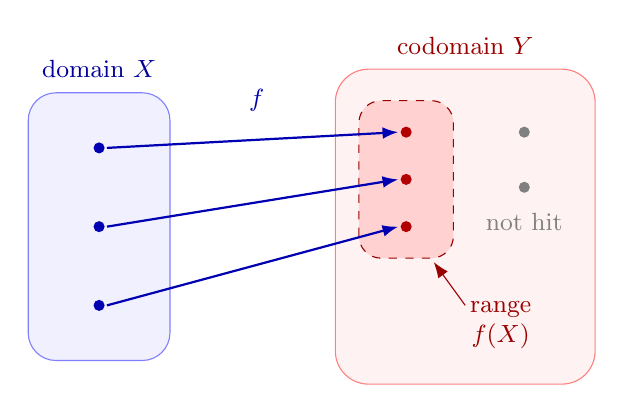
\begin{tikzpicture}[>={Latex[length=2mm]}, every node/.style={font=\small}]
	\draw[rounded corners=10pt, fill=blue!6, draw=blue!50] (-0.9,-1.7) rectangle (0.9,1.7);
	\draw[rounded corners=12pt, fill=red!5, draw=red!50] (3,-2.0) rectangle (6.3,2.0);
	\draw[rounded corners=8pt, fill=red!18, draw=red!60!black, dashed] (3.3,-0.4) rectangle (4.5,1.6);
	\node[blue!60!black] at (0,2.0) {domain $X$};
	\node[red!60!black] at (4.65,2.3) {codomain $Y$};
	\node[red!60!black, align=center] at (5.1,-1.25) {range\\ $f(X)$};
	\draw[red!60!black, ->] (4.65,-1.0) -- (4.25,-0.45);
	\foreach \y in {1.0, 0, -1.0} {\fill[blue!70!black] (0,\y) circle (2pt);}
	\foreach \y in {1.2, 0.6, 0.0} {\fill[red!70!black] (3.9,\y) circle (2pt);}
	\fill[red!40] (4.9,-1.7) circle (0pt);
	\fill[gray] (5.4,1.2) circle (2pt);
	\fill[gray] (5.4,0.5) circle (2pt);
	\draw[->, blue!70!black, thick] (0.1,1.0) -- (3.8,1.2);
	\draw[->, blue!70!black, thick] (0.1,0) -- (3.8,0.6);
	\draw[->, blue!70!black, thick] (0.1,-1.0) -- (3.8,0.0);
	\node[blue!70!black] at (2,1.6) {$f$};
	\node[gray, anchor=north] at (5.4,0.3) {not hit};
\end{tikzpicture}
\end{document}
